\documentclass[11pt]{amsart}
\usepackage{geometry}                % See geometry.pdf to learn the layout options. There are lots.
\geometry{a4paper}                   % ... or a4paper or a5paper or ...
%\geometry{landscape}                % Activate for for rotated page geometry
\usepackage[parfill]{parskip}    % Activate to begin paragraphs with an empty line rather than an indent
\usepackage{enumitem}
\usepackage{graphicx}
\usepackage{amssymb}
\usepackage{amsmath}
\usepackage{cancel}
\usepackage{epstopdf}
\DeclareGraphicsRule{.tif}{png}{.png}{`convert #1 `dirname #1`/`basename #1 .tif`.png}
\usepackage{breqn}
\usepackage{float}
\usepackage{breqn}

\title{Econ 210C Problem Set \# 4}
\author{Minki Kim}
%\date{}                                           % Activate to display a given date or no date

\begin{document}




\maketitle

\section{Labor supply problem}
An individual with time-separable utility solves the following maximization problem: 
\begin{equation*}
\mathcal{L} = \sum_{t=0}^{\infty} \beta^t \bigg( \log C_t + \log (1-L_t)  + \lambda_t  \left(  w_t L_t - C_t \right) \bigg)
\end{equation*}
The first order conditions of the individual are: 
\begin{align*}
\frac{1}{C_t} &= \lambda_t  \\
\lambda_t w_t &= \frac{1}{1-L_t} 
\end{align*}
On the other hand, an individiual with non-separable preferences solves the following dynamic maximization problem :
\begin{equation*}
\mathcal{L} = \sum_{t=0}^{\infty} \beta^t \bigg( \log C_t + \log\left( 1 - 0.5 \left[ L_t + L_{t-1} \right] \right) + \lambda_t  \left(  w_t L_t - C_t \right)  \bigg)
\end{equation*}
The first order conditions for this individual are: 
\begin{gather*}
\frac{1}{C_t} = \lambda_t  \\
\lambda_t w_t = \frac{0.5}{1 - 0.5 \left( L_t + L_{t-1} \right)} + \beta \frac{0.5}{1 - 0.5 \left( L_{t+1} + L_t \right)}
\end{gather*}
\begin{enumerate}[label=(\alph*)]
	\item I assume that there is no means for individuals to save in the economy. Hence, the budget constraint $w_t L_t = C_t$ is satisfied every period. Then, for an individual with separable utility, labor supply is just 
	\begin{equation*}
	L_t = \frac{1}{2}
	\end{equation*}
	Therefore, labor supply does not respond to shocks in this case. Now consider the labor supply for an individual with non-separable preferences. Labor supply for those individuals is characterized by the following equation:
	\begin{equation*}
	\frac{w_t}{C_t}  = \frac{0.5}{1 - 0.5 \left( L_t + L_{t-1} \right)} + \beta \frac{0.5}{1 - 0.5 \left( L_{t+1} + L_t \right)}
	\end{equation*}
	When the positive shock is expected to hit the economy in period $t$, the individual can adjust her labor supply not just in period $t$, but period $t-1$ and $t+1$. For instance, in the wake of negative shock, the individual can choose to work less in period $t$ (when the negative shock is in effect) and work more in the adjacent two periods. Therefore, compared to the case when the utility was separable, labor supply changes are larger to the same shock. 
	
	\item Since $L_t = \frac{1}{2}$ for the separable preferences, labor supply is perfectly inelastic ($\varepsilon_{L,w} = 0$). One would generate higher value of labor supply elasticity by introducing non-separability to preferences. 
\end{enumerate}
\section{Demand shock}
\begin{enumerate}[label=(\alph*)]
	\item A representative consumer solves the following utility maximization problem: 
	\begin{equation*}
	\mathcal{L} = \sum_{t=0}^{\infty} \beta^t \left[ \log C_t - \nu_t \frac{L_t^{1 +\chi}}{1+\chi} + \lambda_t \left( W_t L_t + (P_t + d_t) K_t + \Pi_t - C_t - P_t K_{t+1} \right) \right]
	\end{equation*}
	The first order conditions are: 
	\begin{align*}
	\frac{1}{C_t} &= \lambda_t \\
	\nu_t L_t^\chi &= \lambda_t W_t \\
	\lambda_t P_t &= \beta \mathbb{E}_t \lambda_{t+1} \left(  P_{t+1} + d_{t+1} \right)  \\
	P_t K_{t+1} + C_t & = W_t L_t + (P_t + d_t) K_t + \Pi_t
	\end{align*}
	
	\item Suppose the representative consumer reduces one unit of consumption today and invest those forgone amount of consumption into capital. By giving up one unit of consumption today, the consumer incurs a marginal loss in utility: $\lambda_t$. 
	
	However, the consumer now can use increased amount of capital the next period. Additional amount of capital generates additional amount of dividend net the cost paid to purchase the additional capital in period $t$, which is captured by $\frac{d_{t+1}}{P_t}$, which can be converted to utility term by multiplying $\lambda_{t+1}$. On top of this, the consumer can enjoy a capital gain or incur a capital loss depending on how the price of capital changes from $t$ to $t+1$. This is captured by $\frac{P_{t+1}}{P_t}$. Finally, all these gains are discounted by $\beta$ because they are realized in period $t+1$. In conclusion, we get 
	\begin{equation*}
	\lambda_t = \beta \mathbb{E}_t \frac{\lambda_{t+1} (P_{t+1} + d_t)}{P_t}
	\end{equation*}
	
	\item Capital market is cleared at $K_t^d = K_t^s$. Capital demand is not specified in this model, because we did not specify the supply side of the economy. Capital supply follows the Euler equation obtained in (b). Consumers supply capital up to the point where marginal benefit of additional supply of capital is equal to the marginal cost of giving up consumptions. 
	
	\item The representative consumer's labor supply schedule is: 
	\begin{equation*}
	L_t = \left( \frac{\lambda_t W_t}{\nu_t} \right)^{\frac{1}{\chi}}
	\end{equation*}
	The shock $\nu_t$ is interpreted as a labor disutility shock (or generally preference / taste shock). Higher values of $\nu_t$ increases the disutility of labor supply, hence reduces the labor supply of the consumer. To see how the change of $\nu_t$ affects the labor supply curve, consider a simple case where $\chi = 1$. Then labor supply curve is characterized as: 
	\begin{equation*}
	W_t = \frac{\nu_t}{\lambda_t} L_t = \nu_t C_t L_t  
	\end{equation*}
	Hence, a positive $\nu_t$ shock makes the labor supply curve steeper. 
	
	\item With a strongly countercyclical $\nu_t$, the real wage can be acyclical or even countercyclical even when the consumption and labor supply are procyclical. One of the puzzles that the RBC model generates is that real wage is too procyclical. Introducing $\nu_t$ can solve this problem, but preference shock is hard to justfy.  
\end{enumerate}
\section{Business cycle and external returns to scale}
\begin{enumerate}[label=(\alph*)]
	\item An individual firm $i$'s labor demand is: 
	\begin{equation*}
	\left.\begin{array} { c } { \max _ { K _ { t } ,L _ { i } } E _ { t } K _ { i t } ^ { \alpha } \left( Z _ { t } L _ { i t } \right) ^ { 1- \alpha } - W _ { t } L _ { i t } - d _ { t } K _ { i t } } \\  \rightarrow { W _ { t } = ( 1- \alpha ) \frac{Y_{i,t}}{L_{i,t}} } \end{array} \right.
	\end{equation*}
	\item Since all firms are identical, aggregate production funciton is:
	\begin{align*}
	Y_t &= \int_{0}^{1} E_t K_{i,t}^\alpha \left( Z_t L_{i,t} \right)^{1-\alpha} di \\
	& = E_t Z_t^{1-\alpha} \int_{0}^{1} K_{i,t}^\alpha  L_{i,t}^{1-\alpha} di \\
	& = E_t K_t^\alpha (Z_t L_t)^{1-\alpha}
	\end{align*}
	Using that $E_t = Y_t^{1- \frac{1}{\gamma}}$, we can show that the aggregate production function exhibits increasing returns to scale. 
	\begin{equation*}
	Y _ { t } = \left[ K _ { t } ^ { \alpha } \left( Z _ { t } L _ { t } \right) ^ { 1- \alpha } \right] ^ { \gamma }
	\end{equation*}
	Hence the social labor demand curve is $W _ { t } = \gamma ( 1- \alpha ) Y _ { t } L _ { t } ^ { - 1}$. There is no economic profit in individual firm level, because an individual firm does not have pricing power (perfect competition). We need imperfect competition to generate economic profit in individual firm level. 
	\item We want to see if the model can explain key stylized facts about business cycles: macroeconomic comovement. The model is consistent with these stylized facts. Consider a negative $\nu_t$ shock. Since the consumer feels less disutility from labor, labor supply increases. Since increased labor supply brings more income to the consumer, consumption increases as well. Cyclicality of real wages is a bit ambiguous, because the presence of externalities makes social labor demand flatter. However, if the size of the externalities is moderate so that the social labor demand curve is still downward sloping, wages also increase. Average labor productivity, as measured by $Y_t/L_t$, is also procyclical bercause it's a linear function of real wages. 
	
	\item With $\gamma = 1$, the model reduces to a standard RBC model. Without externalities, the model is unable to generate a flattened social labor demand curve. As a result, real wages and labor productivity become too procyclical. 
	
	\item The statement from the helpless RBC modeler is correct, because in a standard RBC model there is no internal mechanism to suppress the strong procyclicality of wage (and equivalently, labor productivity). The researcher might introduce the preference shock $\nu_t$ in the model, along with the condition $\rho (\nu_t, Z_t) < 0$. Since a negative $\nu_t$ shock makes labor supply curve flatter, the researcher can attain smaller volatilies for wages and larger volatilities for aggregate labor. 
	
	Is this story convincing? A crucial assumption here is the condition $\rho (\nu_t, Z_t) < 0$. In words, this condition implies that when a positive technology shock realizes consumers also feel less disutility from working. People being less 'lazy' in an economic boom does not sound that plausible. According to this story, what happened to the United States in the 1930s was a severe attack of contagious laziness!\footnote{Quote from Franco Modigliani}
	
	The researcher does not need to resort to $\nu_t$ when the economy exhibits $\gamma > 1$. Since the presence of externalities makes social demand curve flatter, the model can generate mildly procyclical wage and labor productivity for reasonable degree of externalities. 
	
	
\end{enumerate}
\section{Problems from Romer's textbook}
\subsection{Problem 6.10}
\begin{enumerate}[label=(\alph*)]
	\item Using the given three equations, it is easy to get the closed form solution for $p, p^{*}$, and $y$. 
	\begin{align*}
	p & = \frac{f \phi m'}{1 - f + f\phi} \\
	p^{*} & = \frac{\phi m'}{1 - f + f\phi} \\
	y & = \frac{m' (1-f)}{1 - f + f\phi}
	\end{align*}
	\item The following figure summarizes the results
	\begin{figure}[H]
		\centering
		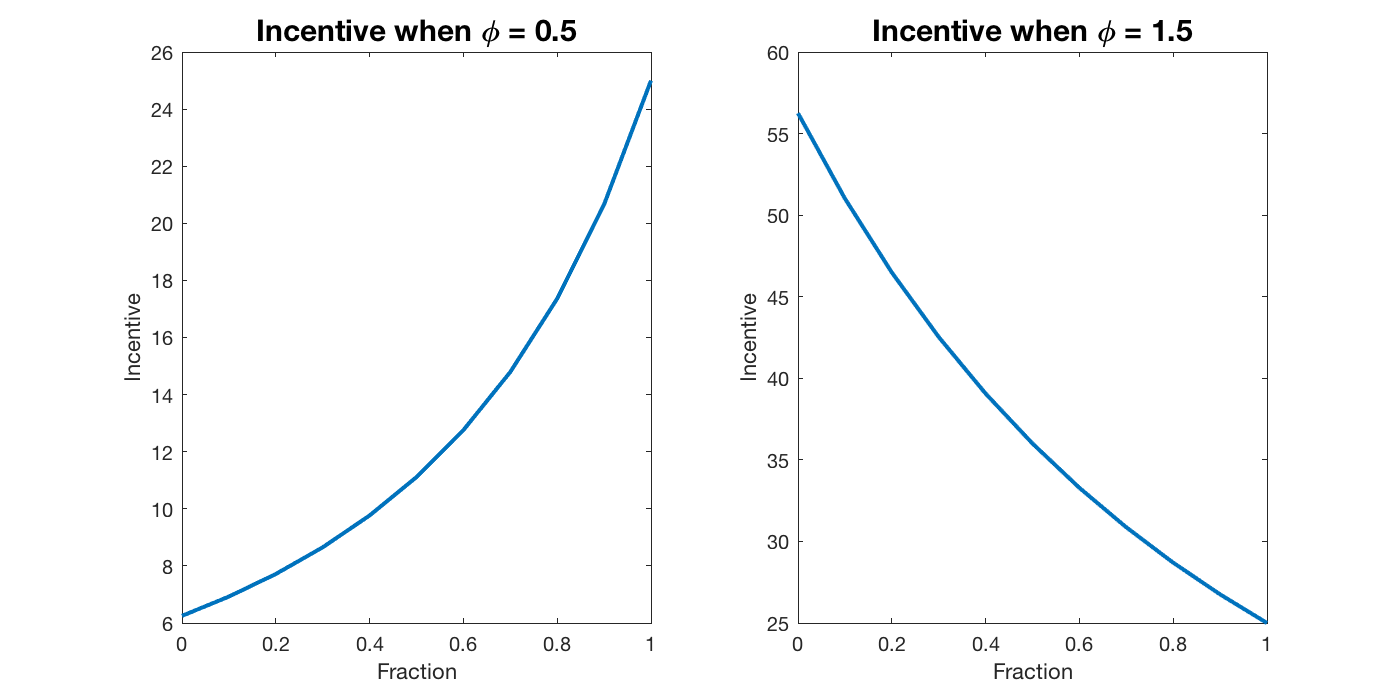
\includegraphics[width=0.85\textwidth]{611b}
		\caption{A firm's incentive to adjust its price}
	\end{figure}
	\item Whether a firm adjusts its price or not depends on the size of the menu cost, $Z$. Assume that $\phi <1$. Now suppose the menu cost is very low, lower than the incentive of a firm when no other firm is adjusting their prices. In this case, all firms adjusting their prices can be a Nash equilibrium. 
	
	Suppose, on the other hand, the case when the menu cost is really high, higher than the incentive of a firm when all the other firms are adjusting their prices. In this case, no price adjustment is the only Nash equilibrium. 
	
	Now suppose that the size of the menu cost lies somewhere between the above two extremes. Specifically, say that $Z = K p^{*} (f)$ for some $f$. Then, a fraction $f$ of the firms adjusting their prices is the only Nash equilibrium, because for $f' \neq f$ some firms have incentives to deviate from adjusting (not adjusting) prices. 
\end{enumerate}
\subsection{Problem 6.11}
\begin{enumerate}[label = (\alph*)]
	\item If the firm does not adjust its price and stays at $r^{*}(y_0)$ level, its profit is $\pi \left( y_1, r^{*}(y_0)  \right)$. On the other hand, if the firm choose to adjust its price to the optimal level for $y_1$, its profit is $\pi \left( y_1, r^{*}(y_1)  \right)$ The difference between these two is a potential gain from adjusting the price, so can be interpreted as the incentive to adjust its price. The smaller $G$ is, the stickier prices are. 
	
	\item Now we have
		\begin{align*}
		\begin{split}
		\frac{\partial^2 G}{\partial y_1^2} = \pi_{11}(y_1, r^*(y_1))  &+ \pi_{12}(y_1, r^*(y_1)) \frac{\partial r^*(y_1)}{\partial y_1} + \left(\pi_{21}(y_1, r^*(y_1)) \\
		&+ \pi_{22}(y_1, r^*(y_1)) \frac{\partial r^*(y_1)}{\partial y_1} \right) \frac{\partial r^*(y_1)}{\partial y_1} + \pi_2(y_1, r^*(y_1)) \cdot \frac{\partial^2 r^*(y_1)}{\partial y_1^2} - \pi_11(y_1, r^*(y_0))
		\end{split}
		\end{align*}
	but we know
	\[
	\pi_2(y_1, r^*(y_1)) = 0
	\]
	and 
	\[
	\pi_{12} = \pi_{21}
	\]
	so we can evaluate at $y_0$ to get
	\[
	\frac{\partial^2 G}{\partial y_1^2} \vert_{y_0} = 2 \pi_{12}(y_0, r^*(y_0)) \frac{\partial r^*(y_0)}{\partial y} + \pi_{22}(y_0, r^*(y_0)) \cdot \frac{\partial^2 r^*(y_0)}{\partial y^2}
	\]
	
	Implicitly differentiating $\pi_2(y_0, r^*(y_0)) = 0$ gives 
	\[
	\pi_{21} = - \pi_22 \times \frac{\partial r^*(y_0)}{\partial y}
	\]
	which we can substitute to get our Taylor series expansion, which only includes the second order term, as
	\[
	G \approx - \frac{1}{2} \pi_{22}(y_0, r^*(y_0)) \left(\frac{\partial r^*(y_0)}{\partial y}\right)^2 (y_1-y_0)^2
	\]

	\item $\pi_{22}$ is the curvature of the profit function, which captures the degree of insensitivity of the profit function. $r^{*'}(y_0)$ is the degree of real rigidity. It captures how sensitive the optimal price is to changes in output. 
\end{enumerate}
\subsection{Problem 6.12}
\begin{enumerate}[label = (\alph*)]
	\item First, we can substitute our wage expression $w = \theta p$ to get
	\[
	p = \theta p + (1-\alpha) \ell - s \implies p = \frac{(1-\alpha) \ell - s}{1-\theta}
	\]
	and we are given aggregate demand, so we have
	\[
	y = m - p = m - \frac{(1-\alpha) \ell - s}{1-\theta}
	\]
	and from our output equation we have
	\[
	s + \alpha \ell = m - \frac{(1-\alpha) \ell - s}{1-\theta} \implies \ell = \frac{(1-\theta) m + \theta s}{1-\theta \alpha}
	\]
	which we can substitute into our price equation to get
	\[
	p = \frac{(1-\theta) m - s}{1-\theta \alpha}
	\]
	and now we have our output
	\[
	y = \frac{(1-\theta) \alpha m + s}{1-\theta \alpha}
	\]
	and we can find wage using the original wage expression to get
	\[
	w = \theta p = \theta \times \frac{(1-\theta) m - s}{1-\theta \alpha}
	\]
	and we can now find how employment responds to shocks. We can take cross-partial derivatives to obtain:
	\[
	\frac{\partial^2 \ell}{\partial m \partial \theta} = \frac{\alpha - 1}{(1-\theta \alpha)^2}
	\]
	for how indexation moderates the effect of a monetary shock and
	\[
	\frac{\partial^2 \ell}{\partial s \partial \theta} = \frac{1}{(1-\theta \alpha)^2}
	\]
	for how indexation moderates the effect of a supply shock.
	
	Since $\alpha - 1 < 0$, we have that greater indexation reduces the effect of a monetary shock, while $1 > 0$ tell us that greater indexation scales the effects of supply shocks up.
	
	\item With independence we can just use the formula for the variance of a linear combination of two random variables. So we have
	\begin{align*}
	Var(\ell) = \left(\frac{1-\theta}{1-\theta \alpha}\right)^2  \quad Var(m) + \left(\frac{\theta}{1-\theta \alpha}\right)^2 Var(s)
	\end{align*}
	Take the partial derivative of this with respect to $\theta$ to get the first order condition: 
	\[
	(1-\theta)(\alpha-1) Var(m) + \theta Var(s)
	\]
	so solving for $\theta$ we get
	\[
	\theta^* = \frac{(1-\alpha) Var(m)}{(1-\alpha) Var(m) + Var(s)}
	\]
	as the wage indexation that minimizes employment variance.
	
	\item \begin{enumerate}[label = (\roman*)]
		\item We can easily see that we have
		\[
		y_i - y = \alpha (\ell_i - \ell) \implies \ell_i = \ell + \frac{y_i - y}{\alpha} = \ell - \frac{\theta_i - \theta}{\alpha} \times \phi p
		\]
		and we already have expressions for employment and the price levels that we can substitute to get
		\[
		\ell_i = \frac{(1-\theta) \alpha - \phi (1-\alpha) (\theta_i - \theta)) m + (\theta \alpha + \phi (\theta_i - \theta)) s}{(1-\theta \alpha) \alpha}
		\]
		for employment at firm $i$.
		
		\item We now have
		\[
		\operatorname{Var}(\ell_i) = \left(\frac{(1-\theta) \alpha - \phi (1-\alpha) (\theta_i - \theta)}{(1-\theta \alpha) \alpha}\right)^2 \operatorname{Var}(m) + \left(\frac{\theta \alpha + \phi (\theta_i - \theta)}{(1-\theta \alpha) \alpha}\right)^2 \operatorname{Var}(s)
		\]
		so we must satisfy the first order condition
		\[
		(\alpha - 1) \phi [(1-\theta) \alpha - \theta_i (1-\alpha) \phi + \theta (1-\alpha)] \operatorname{Var}(m) + \phi[\theta \alpha + \phi \theta_i - \phi \theta] \operatorname{Var}(s) = 0
		\]
		which allows us to solve for $\theta_i$ to get
		\[
		\theta_i^* = \frac{(1-\alpha) \phi ((1-\theta)\alpha + \theta \phi (1-\alpha)) \operatorname{Var}(m) + \phi \theta(\alpha - \phi) \operatorname{Var}(s)}{(\phi(1-\alpha))^2 \operatorname{Var}(m) + \phi^2 \operatorname{Var}(s)}
		\]
		
		\item The Nash equilibrium value implies that each firm's first order condition can have $\theta_i$ and $\theta$ identical. So we need 
		\[
		(\alpha - 1) \phi [(1-\theta) \alpha - \theta (1-\alpha) \phi + \theta (1-\alpha)] \operatorname{Var}(m) + \phi[\theta \alpha + \phi \theta - \phi \theta] \operatorname{Var}(s) = 0
		\]
		which simplifies to 
		\[
		(1-\theta) \alpha (1 - \alpha) \phi \operatorname{Var}(m) - \theta \alpha \phi \operatorname{Var}(s) = 0
		\]
		allowing us to solve for the Nash value of $\theta$ as
		\[
		\theta_{\text{Nash}} = \frac{(1-\alpha) \operatorname{Var}(m)}{(1-\alpha) \operatorname{Var}(m) + \operatorname{Var}(s)}
		\]
		which is the same value as in part b.
	\end{enumerate}
\end{enumerate}

\end{document}
